\chapter*{Forord}

Automatisk orddeling er en viktig del av dagens systemer for tekstsetting. Dessverre skjer det ikke uten feil. Nærmest daglig kan vi i aviser og nettpublikasjoner se eksempler på uheldig orddeling, som fører til misvisende eller komiske ordbilder -- eksempelvis som i figur~\ref{fig:forord-doplager}. Dette vil være et økende problem i den hektiske mediehverdagen, hvor nyheter må publiseres raskt og korrekturarbeid nedprioriteres. \TeX{}\sidenote[-5]{\TeX{}, utviklet av Donald Knuth, er et program for spesifisering av layout og typografisk tekstsetting.}, og er et av de fremste, fritt tilgjengelige systemene for tekstsetting. Programmet finner omtrent 90~\% av alle lovlige delepunkter, med rundt én prosent gale delinger \cite{thoresen1993virtuelle}. I majoriteten av tilfellene trengs det kun ett delepunkt når et ord må deles ved linjeslutt. Det er derfor viktigst at antall gale delinger reduseres fremfor å finne flest mulige av de lovlige delepunktene i et ord. Sett i lys av dette fungerer \TeX{}-algoritmen godt. Et større problem er at orddelingsalgoritmen i \TeX{} først og fremst er utviklet med tanke på amerikansk-engelsk orddeling, som er basert på uttale. Systemet har ingen støtte for \term{ikke-standard orddeling}\sidenote[-11]{Ikke-standard orddeling betegner orddelingsregler som avviker fra den typiske orddelingen hvor en bindestrek skytes inn mellom to bokstaver i ordet. Et eksempel er ord som endrer stavelse ved orddeling. I tysk finnes «backen» som skal deles som «bak-ken», eller i norsk hvor «soppose» blir til «sopp-pose».}. Dette er et problem som gjelder de fleste, også kommersielle, systemer for tekstsetting. Et tredje problem er den manglende kontrollen over orddeling som tilbys i alle dagens systemer. For norsk skriftspråk har vi flere regler som kan gi opphav til delepunkter i et ord. Disse kan argumenteres for å være av varierende kvalitet. Det vil derfor være ønskelig å kunne skille mellom typer av orddelingsregler som skal benyttes ved orddeling. Vi har i hovedsak to regler for orddeling: \term{ordleddsregelen} og \term{enkonsonantregelen}. Ordleddsregelen sier at vi skal dele ord «mellom betydningsbærendebærende og/eller lett gjenkjennelige orddeler», og benyttes i hovedsak ved sammensatte ord, avledninger og bøyningsendelser. Enkonsonantregelen forteller: «uavhengig av ordets betydning, la én konsonant følge med til neste linje». \cite{vinje} Ut fra dette ser vi at orddelingen i figur~\ref{fig:forord-freskukens} er lovlig, men også uheldig. Ved å benytte ordleddsregelen ville dette vært unngått. For sammensatte ord vil ordleddsreglen, fremfor enkonsonantregelen, typisk føre til færre misvisende delinger. Men dessverre tilbyr ingen av dagens metoder for automatisk orddeling en slik grad av kontroll. I denne oppgaven ser vi nærmere på disse problemene og muligheten for å utvikle en løsning.

\marginelement[-21]{

\includegraphics[width=\marginparwidth]{content/figures/forord-doplager.jpg}
\captionof{figure}[Uheldig orddeling]{Eksempel på uheldig orddeling som fører til et komisk ordbilde. 
Faksimile, Dagbladet nett 25. september 2013.  \url{http://www.dagbladet.no/2013/09/25/nyheter/utdanning/narkotika/innenriks/29445603/}}
\label{fig:forord-doplager}
}


\marginelement[-5]{
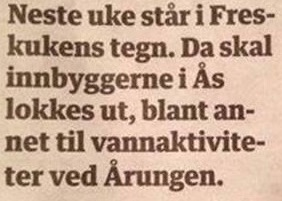
\includegraphics[width=\marginparwidth]{content/figures/forord-freskukens.jpg}
\captionof{figure}[Uheldig bruk av enkonsonantregelen]{Eksempel på uheldig bruk av enkonsonantregelen, som ga opphav til et komisk ordbilde.
Faksimile, Østlandet Blad.}
\label{fig:forord-freskukens}
}

\clearpage

Målet for oppgaven er å skissere og implementere et analytisk system, som kan dele ord etter de gjeldene reglene for orddeling, samtidig gi kontroll over reglene som skal benyttes. For å få til dette er det flere individuelle oppgaver som må løses, og systemet vil få en modulbasert arkitektur. I forbindelse med dette har jeg spesielt to spørsmål jeg ønsker svar på, og har formulert følgende problemstillinger (PS):

\begin{quote}
PS1: Hvor godt utfører modulene oppgavene sine hver for seg?
\end{quote}

Det vil være interessant å se nærmere på modulene i isolasjon med egne testkriterier og tester. Med dette vil det være mulig å identifisere svakheter i enkeltmoduler i programflyten, og kan fungere som en pekepinn på mulig videre arbeid for å forbedre programmet.

\begin{quote}
PS2: Hvor god kvalitet og kontroll får vi på orddelingen?
\end{quote}

Her ønsker vi å få svar på hvor vellykket løsningen er for å dele ord, samt hvilken eventuell økt kontroll vi kan få over orddelingsvalgene.

\section*{Takksigelser}

Først og fremst vil jeg gjerne takke min veileder Dag Langmyhr for å ha gitt så mye av sin tid og for spennende samtaler, rundt det som for mange er et smalt tema. Jeg vil også takke kjæresten min for korrekturlesning og støtte under en intens innspurt. Til sist -- takk til familie og venner for inspirasjon og gledelige stunder!